\chapter{V-rep Simulation}
\label{crashcourse}

The robotic control lab (3071 ECEB) receives a large volume of students with the expansion of ECE470 and ECE489. Lab space and work benches can be in high demand toward the end of the semester. Therefore, we highly encourage students to build and test your robot algorithms in simulation environments before deploying them on actual robots to relieve lab usage. Although any simulation software and environment that serve this purpose are welcomed, we recommend \textit{V-rep} for those of you who don't have any preference. \textit{V-rep} is a robot simulator with integrated development environment that is avaliable in Windows, Mac os, and Linux. Within \textit{V-rep}'s simulation environment, each object/model can be individually controlled via an embedded script, a ROS node, or a remote API client. And the script that is used to control robots in simulation can be written in C/C++, Python, Java, Lua, Matlab or Octave. These features make \textit{V-rep} adapt well to this course well and give students lots of freedom when conducting their own robot experiments without a physical robot. 

\section{Download and Install V-rep on your PC}
\begin{itemize}
\item Download the latest version of V-REP PRO EDU that suits your PC's operation system from: \url{http://www.coppeliarobotics.com/downloads.html}
\end{itemize}

\begin{figure}[h]
\centering
	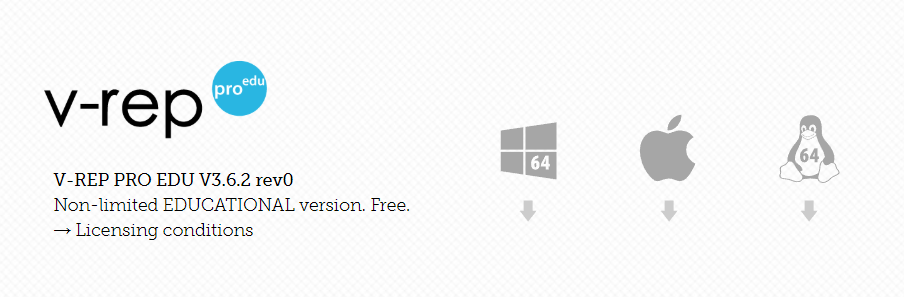
\includegraphics[scale=0.55]{appendixB_vrep_download.png}
\caption{\figlbl{downloadvrep}Download the latest version of V-REP PRO EDU}
\end{figure}

\begin{itemize}
\item For Windows users, launch and install the setup.exe file on your computer. It seems \textit{V-rep} prefers to be installed on C drive.
\item For Mac users, unzip the V-REP\_PRO\_EDU\_Vx\_x\_x\_Mac.zip folder and rename it if you prefer. Open a terminal inside the unzipped folder directory and type this command: 
\begin{lstlisting}[language=bash]
$ ./vrep.app/Contents/MacOS/vrep
\end{lstlisting}
\item For Linux users, unzip the V-REP\_PRO\_EDU\_Vx\_x\_x.tar folder and rename it if you prefer. Open a terminal inside the unzipped folder directory and type this command: 
\begin{lstlisting}[language=bash]
$ ./vrep.sh
\end{lstlisting}
\item To learn more about using \textit{V-rep} via command lines, visit:
\url{http://www.coppeliarobotics.com/helpFiles/en/commandLine.htm}
\end{itemize}

\section{Setup remote API to interface with V-rep}
\begin{itemize}
\item Follow instructions on \url{http://www.coppeliarobotics.com/helpFiles/en/remoteApiClientSide.htm} to enable the remote API with the programming language you prefer. (We recommend Python for ECE470)

\item You will be saving your remote API code in a different directory (any directory you want but preferably not the directory that contains \textit{V-rep}'s main program). For example, if you are using Python, create a new directory with a name you like, this new directory must contain the following files (besides the .tttt scene file and your Python remote API script) for the remote API function to work (See \figref{vrepwd}):

\textbf{vrep.py}

\textbf{vrepConst.py}

\textbf{remoteApi.dll, remoteApi.dylib or remoteApi.so} (depends on your operation system)

\end{itemize}

\begin{figure}[h]
\centering
	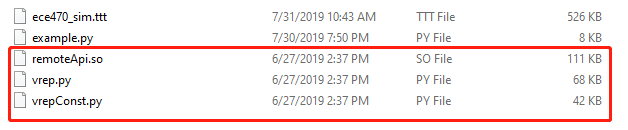
\includegraphics[scale=0.7]{appendixB_vrep_folder.png}
\caption{\figlbl{vrepwd}An example of a working directory}
\end{figure}

\begin{itemize}
\item If you are a Python 3 user, we do have a remote API starter code for you to play with:
\url{http://coecsl.ece.illinois.edu/ece470/ece470_vrep_Linux.zip}
\url{http://coecsl.ece.illinois.edu/ece470/ece470_vrep_Win64.zip}
\end{itemize}

\section{Add a robot in your scene}
\begin{itemize}
\item Drag any robot of interest from the menu on the left hand side to the scene.

\end{itemize}
\begin{figure}[h]
\centering
	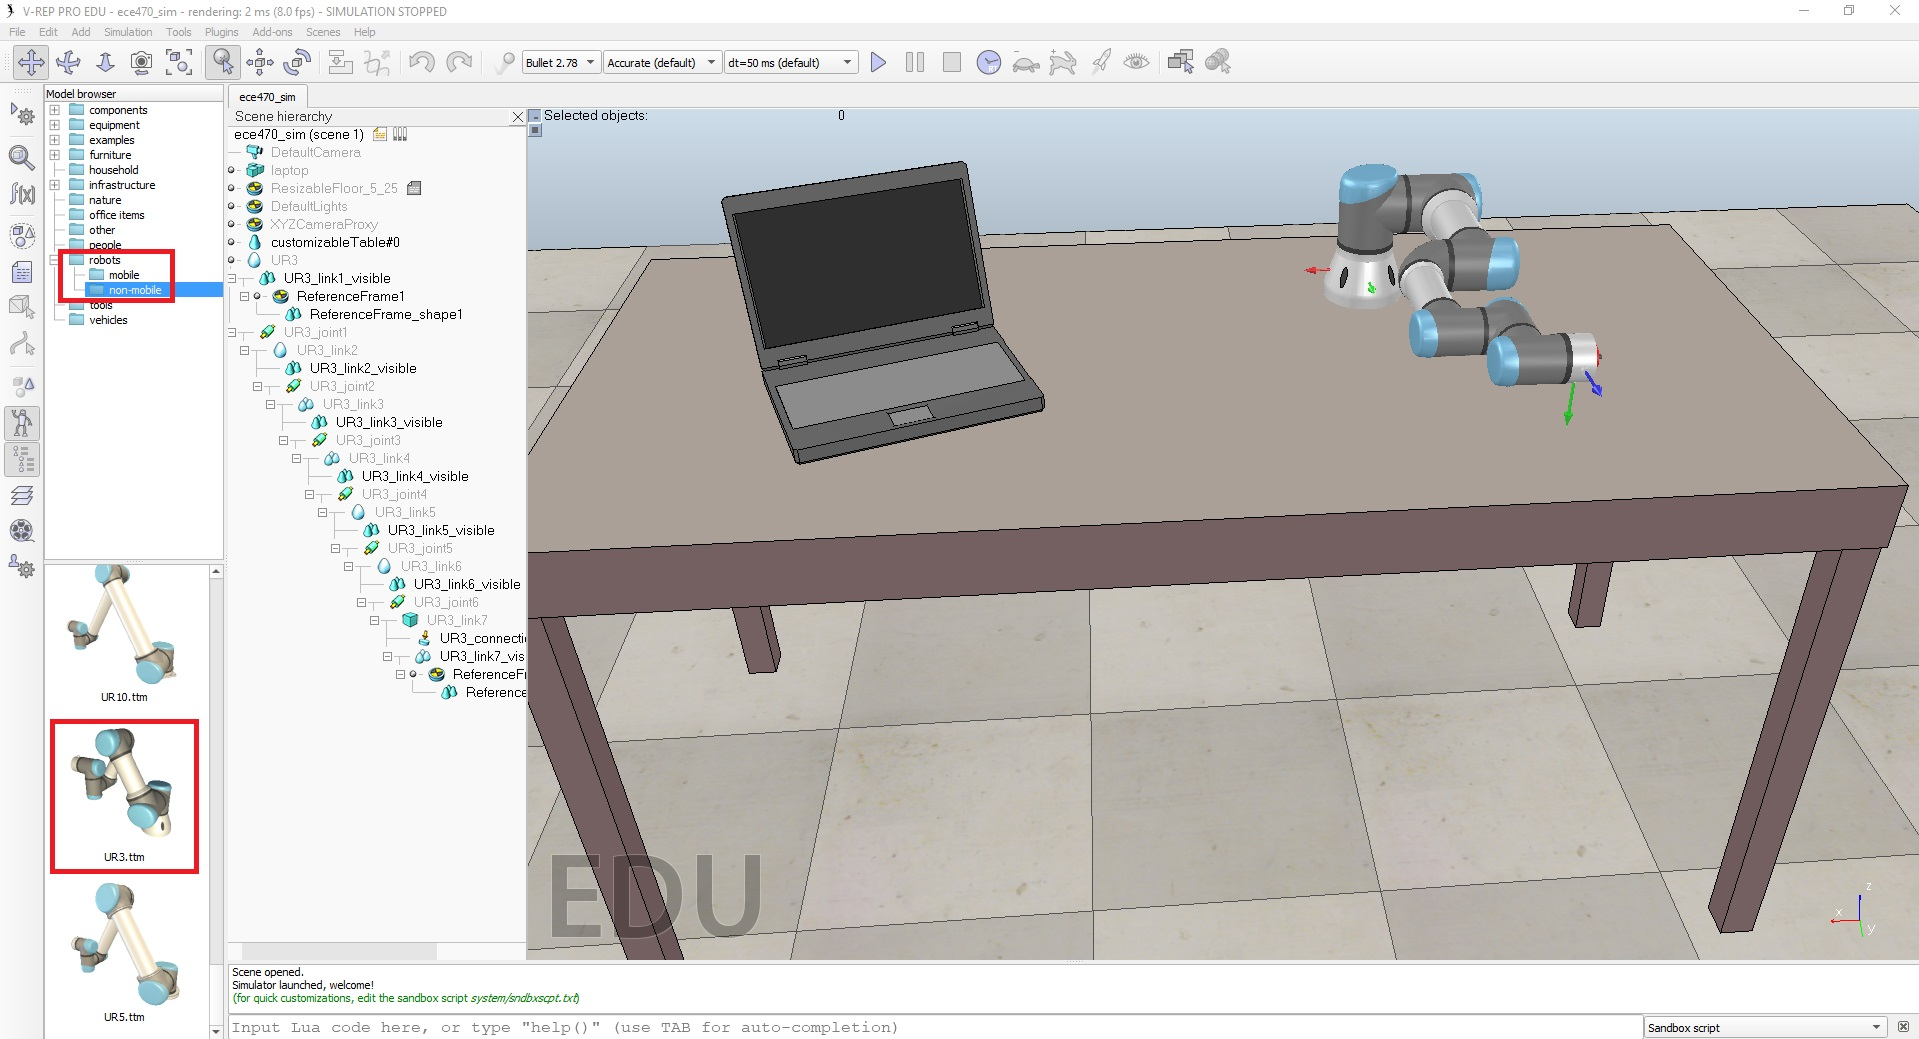
\includegraphics[scale=0.2]{appendixB_vrep_robot.jpg}
\caption{\figlbl{vrepadd}Adding robot to your scene}
\end{figure}
\begin{itemize}

\item Re-position the robot using the move and rotate icons locate on the top menu bar.

\item Delete the default child script (\figref{vrepdelete}) from your robot before you try your remote API program, otherwise you will have two scripts that control the same robot.
\item Save the scene you created as .tttt file in the directory that contains your remote API script.
\end{itemize}

\begin{figure}[h]
\centering
	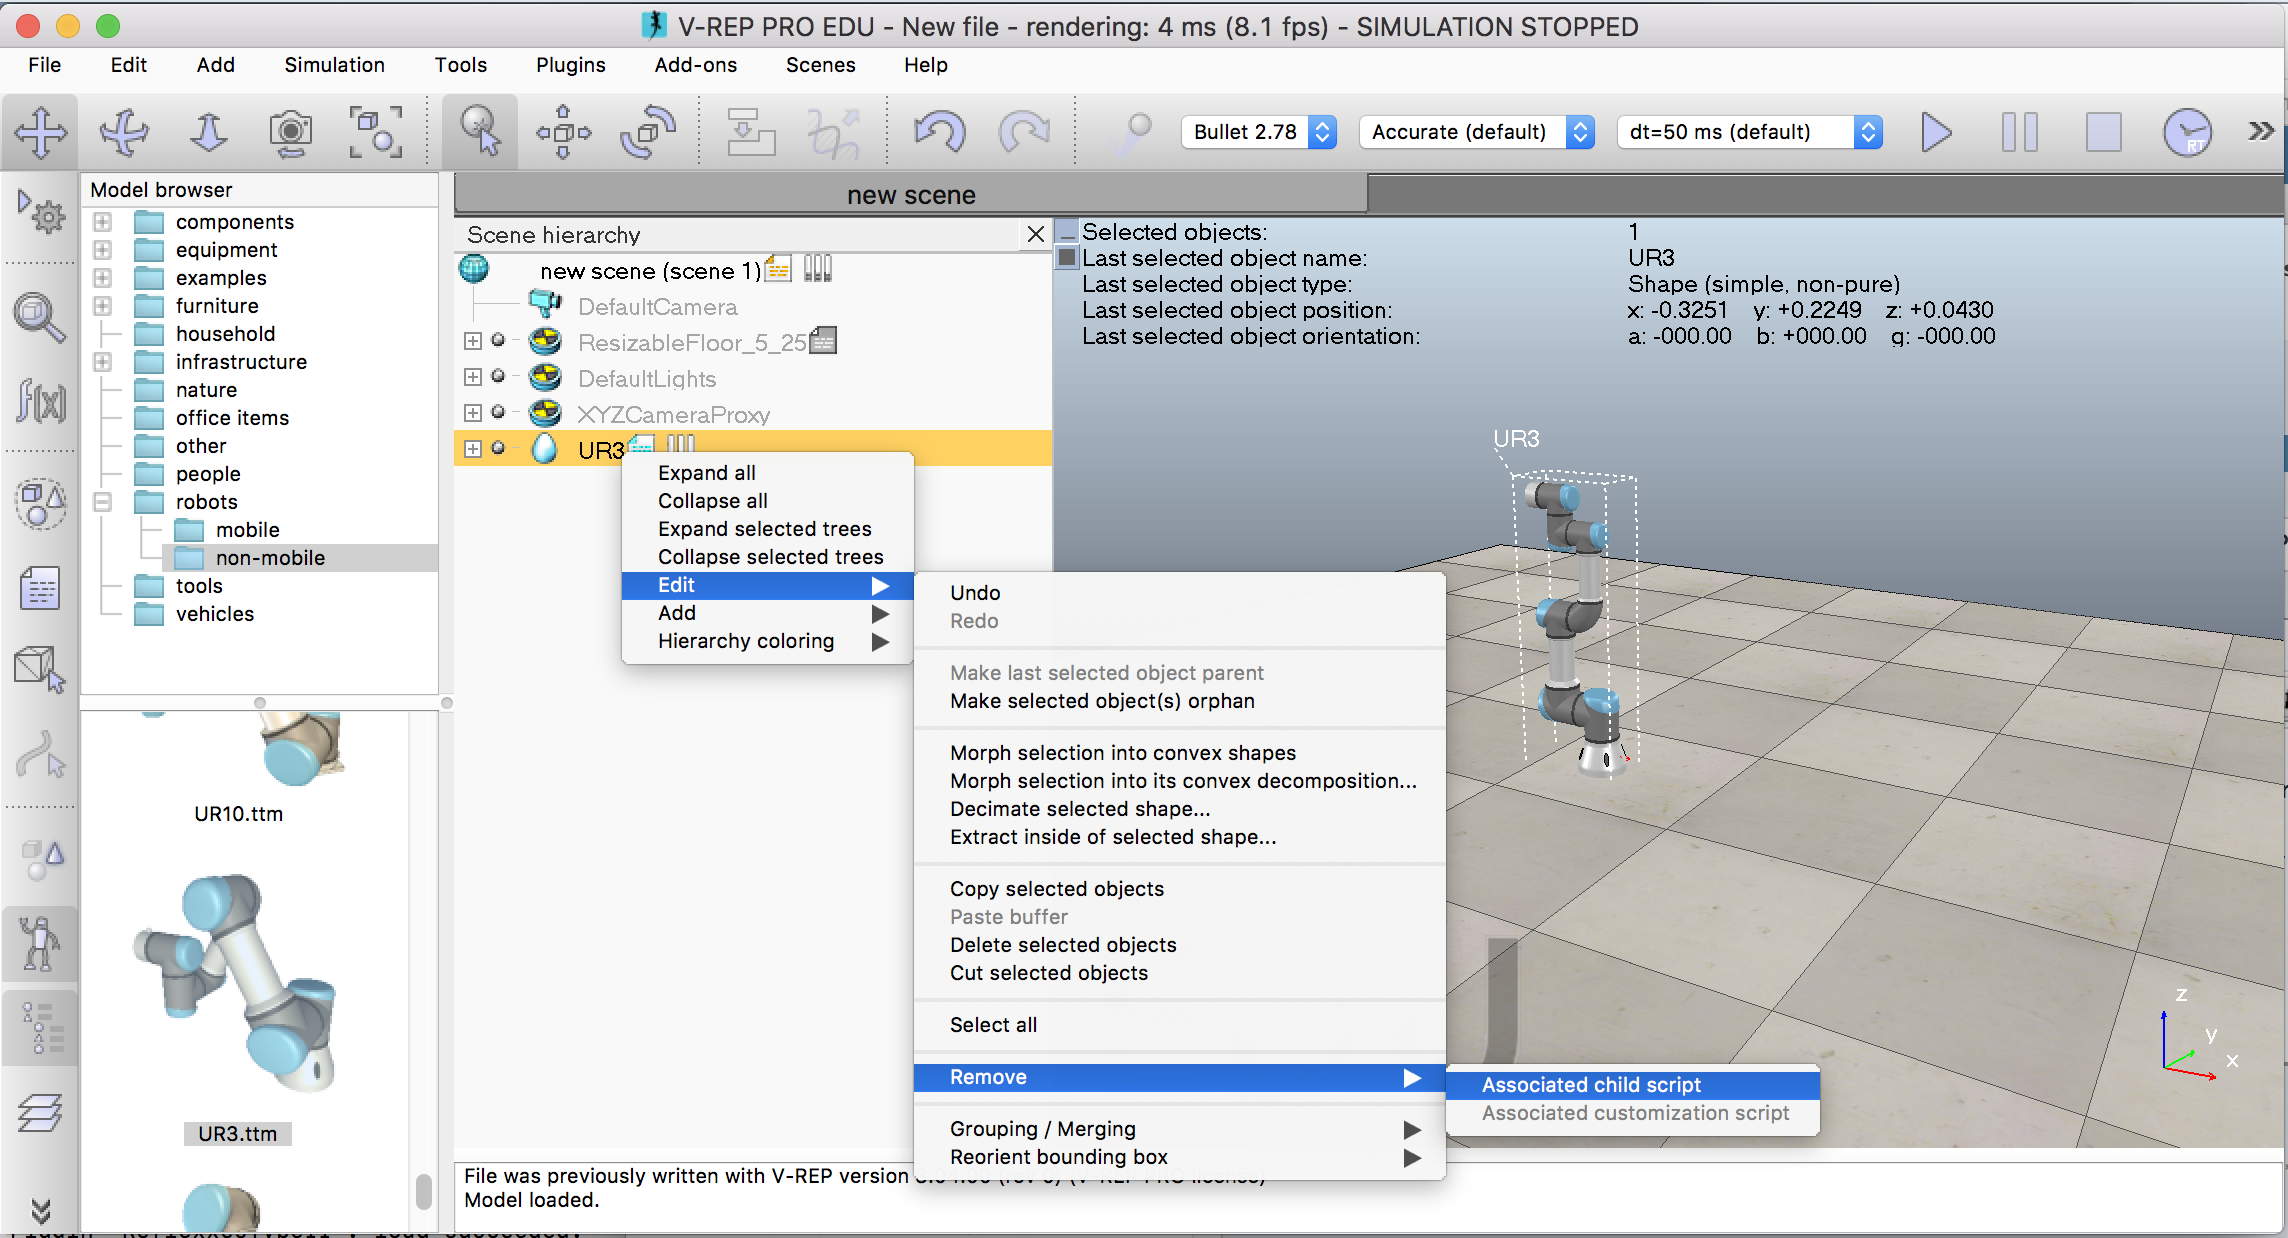
\includegraphics[scale=0.3]{appendixB_Add_ur3.png}
\caption{\figlbl{vrepdelete}Delete the default child script from ur3}
\end{figure}


\section{Important notes!!}
\begin{itemize}
\item The dimension of the UR3 in \textit{V-rep} is somewhat different than the actual UR3 we use in lab. Therefore, when building your forward kinematics function in \textit{V-rep}, \textbf{DO NOT} use the dimensions from UR3's engineering drawing. Instead, you can use the following API function:
\begin{lstlisting}[language=bash]
vrep.simxGetObjectPosition()
\end{lstlisting}
to obtain the distance between two joint centers.

\item The drawback of using numerical solvers is the inconsistency between each simulation's result, especially in less significant digits (e.g. ans = 1.2345644 vs. ans = 1.234598). You may add a rounding step after some parameters of interest to reduce the chance of being inconsistent (e.g. round(ans) = 1.2346).

\item For detailed information on \textit{V-rep} API functions:

\underline{\textbf{Python}}

\url{http://www.coppeliarobotics.com/helpFiles/en/remoteApiFunctionsPython.htm}

\underline{\textbf{Matlab}}

\url{http://www.coppeliarobotics.com/helpFiles/en/remoteApiFunctionsMatlab.htm}

\underline{\textbf{C++}}

\url{http://www.coppeliarobotics.com/helpFiles/en/remoteApiFunctions.htm}

\end{itemize}